% Adapted from UH Manoa theme by:
% UH Manoa presentation theme for beamer
% Jeff Delmerico <jeffdelmerico@gmail.com> 2012
% https://github.com/jeffdelmerico/UH_Beamer_Theme.git


\documentclass{beamer}
%\documentclass[handout]{beamer}
\usetheme{PD}

\usepackage[utf8]{inputenc}
\usepackage[absolute,overlay]{textpos}
\usepackage{helvet}
\usepackage{tikz}
\usepackage{listings,lstautogobble}
\usepackage{syntax}
\usepackage{mathrsfs}
\usepackage{amsmath}
\usetikzlibrary{tikzmark,fit,decorations.pathreplacing}
%\usepackage{enumerate}

\title{TCP flavors for mobile and high-speed environments}
\subtitle{\newline Freeze-TCP, TCP-Probing and Compound TCP}
\author{Giovanni Mazzocchin}
\date{September 20th, 2018}
\institute{Università degli Studi di Padova}

\lstset{
	autogobble=true
}

\setlength{\grammarindent}{3em}

\begin{document}

\newcommand{\turnOffNumbers}{true} %hide frame numbers in footer

\begin{frame}[noframenumbering]
\titlepage
\end{frame}

\let\turnOffNumbers\empty
\begin{frame}
	\frametitle{Outline}
	\tableofcontents
\end{frame}

\section{Scenario}
\begin{frame}{Scenario}
	\begin{itemize}
		\item \textbf{TCP} wasn't designed to cope with mobility issues and high-speed networks.
		\item Several enhancements to standard TCP have been devised:
		\begin{itemize}
			\item mobility and power consumption is now taken into account (\textit{I-TCP}, \textit{M-TCP}, \textit{Freeze-TCP});
			\item some enhancements tackle problems posed by high-speed and long-distance networks
			      (\textit{FAST TCP}, \textit{Compound TCP}).
		\end{itemize}
	\end{itemize}
\end{frame}



\section{Freeze-TCP}
\begin{frame}{Previous approaches}
  \begin{itemize}
    \item Many approaches involve base stations in flow and congestion control. Besides, they
    often split the connection (\textit{I-TCP}, \textit{M-TCP}, \textit{Snoop} etc...).

    \item \textbf{Freeze-TCP} is an end-to-end scheme and doesn't require the involvement of any
        intermediaries for flow control.
    \item In order to achieve \textit{Freeze-TCP}'s goals, changes in TCP code don't go beyond the mobile
          client.
  \end{itemize}
\end{frame}

\begin{frame}{Standard window management}
	\begin{itemize}
		\item When the receiver advertises a zero-size window,
		      the sender enters the \textbf{persist mode}:
		      \begin{itemize}
			    \item \textit{Zero Window Probes} are sent
				  until the receiver's window opens up;
			    \item eventually, the receiver sends back a non-zero window size,
				  and the sender will open its sending window.
		      \end{itemize}
	\end{itemize}
\end{frame}

\begin{frame}{Issues in mobile environments}
	\begin{itemize}
		\item Even if a single packet is dropped due to a short disconnection,
		      standard TCP wrongly thinks that the loss was caused by
		      congestion and chokes the transmission.
		\item Thus, standard TCP's sender unnecessarily holds back,
		      (slow window growth), even
		      though the receiver often recoups quickly from a
                      short disconnection.
	\end{itemize}

	\begin{figure}
                \centering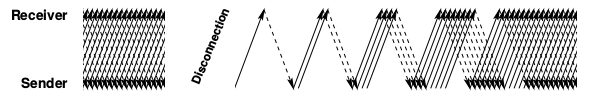
\includegraphics[scale=0.4]{freeze-disconn}
        \end{figure}

\end{frame}

\begin{frame}{Freeze-TCP approach (1)}
	\begin{itemize}
	  \item The mobile client should signal any impending disconnection:
	  \begin{itemize}
		\item this is done via \textbf{signal strength monitoring};
		\item after detecting a disconnection:
		   \begin{enumerate}
			\item the mobile client advertises a zero window size;
			\item the sender switch to \textit{ZWP} mode and
			      doesn't shrink its window.
		   \end{enumerate}
	  \end{itemize}
	\end{itemize}

\end{frame}

\begin{frame}{Freeze-TCP approach (2)}
       \begin{itemize}
		\item How much in advance of the disconnection should the receiver advertise a window size of zero?
		\item There should be a \textit{warning period} prior to disconnection.
		\item They figured out that a sensible choice is the \textit{Round-Trip-Time}:
	           \begin{enumerate}
			\item if it is too long, there will be idle time
			      prior to the disconnection;
			\item if it is too small, the sender's window could
			      drop due to packet losses.
		   \end{enumerate}
       \end{itemize}

\end{frame}


\begin{frame}{Freeze-TCP approach (3)}
       \begin{itemize}
                \item A relevant issue: the \textit{ZWP}s are exponentially backed off,
			so there could be an idle time after a reconnection.
		\item Trick: soon after the reconnection, the receiver
		      sends 3 copies of the ACK for the last data segment
		      it received before the disconnection (\textbf{TR-ACKs}).
       \end{itemize}

       \begin{figure}
                \centering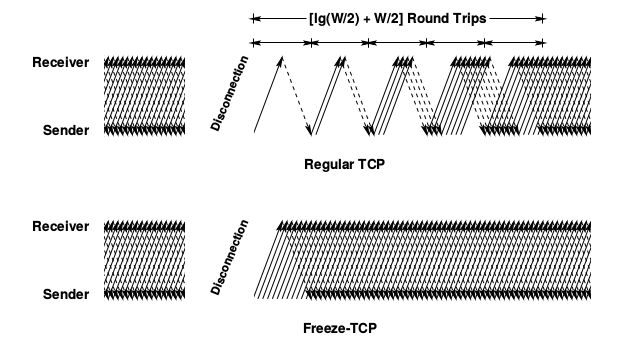
\includegraphics[scale=0.3]{freeze-disconn1}
       \end{figure}

\end{frame}

\begin{frame}{Freeze-TCP approach (4)}
        It can be shown that the (approximate) number
	of extra packets transferred by \textit{Freeze-TCP} is given by:
	$$
		{{W^2 \over 8} + {WlgW} - {5W \over 4} + 1}
	$$
\end{frame}

\begin{frame}{Open issues}
       \begin{itemize}
		 \item In order to apply this protocol, the network stack
		       should be aware of mobility.
		 \item Is it reasonable to restart transmission at the full rate 
		       with the old window size upon entering a new environment?
		\item  The receiver must predict impending disconnections.
       \end{itemize}
\end{frame}



\section{TCP-Probing}
\begin{frame}{Improving energy efficiency}
	\begin{itemize}
		\item Energy efficiency is becoming paramount
		      in communication protocols (a cross-layer issue).
		\item The error control mechanism should
		      be friendly both to \textbf{throughput} and \textbf{low power consumption}.
		\item Energy-conserving capabilities in standard TCP: \newline
		      after segment drops, it shrinks the window so as to
		      save transmission effort.
	\end{itemize}

\end{frame}

\begin{frame}{Improved Error Recovery for \newline better Energy Efficiency}
    \begin{itemize}
	\item The Error Recovery mechanism is not always efficient:
	      in fact, standard TCP thinks that packet losses always happen due to
	      \textit{congestion}.
	\item In case of \textit{infrequent} and \textit{transient} errors,
	      standard TCP strategy leads to:
	      \begin{enumerate}
	      	\item unneeded effective throughput degradation;
		\item increase in overall connection time.
	      \end{enumerate}
	\item Moreover, monitoring network conditions only by means of
	      packet losses causes major energy wastage.
    \end{itemize}
\end{frame}

\begin{frame}{TCP-Probing approach}
   \begin{itemize}
	\item In \textbf{TCP-Probing}, when a segment is dropped, the
	sender initiates a \textbf{probe cycle} (described later).
	\item The \textit{probe cycle}'s duration is naturally extended
	 according to the error condition.
	\item Random losses trigger short probe cycles.
   \end{itemize}
\end{frame}

\begin{frame}{Probe Cycle (1)}
   \begin{itemize}
        \item \textbf{Immediate Recovery}: \newline
	      if network conditions
	      detected when the probe cycle is over are
	      acceptable, the protocol simply restarts from
	      the state before the timeout event.
        \item Otherwise, TCP-Probing opts for \textit{Slow-Start} (conservative
	      approach).
   \end{itemize}
\end{frame}


\begin{frame}{Probe Cycle (2) - Implementation}
   \begin{enumerate}
	\item  The sender transmits \textit{PROBE1}, to which the receiver
    	       immediately responds with \textit{PR1_ACK}. After receiving
	       the latter the sender transmits \textit{PROBE2}.
  	\item  The receiver acknowledges this second probing
	       with a \textit{PR2_ACK} and returns to the \textit{ESTAB} state.
  	\item  A critical part of the probing mechanism is the
    	       protocol's behaviour at the end of the cycle.
   \end{enumerate}
\end{frame}


\begin{frame}{Probe Cycle (3) - Implementation}
   \begin{itemize}
	\item A \textit{measurement timer} is used to measure
	     the two RTTs from the probe cycle.
	\item Upon exiting the probe cycle, the two measured RTTs
	      are compared.
	      \begin{enumerate}
		   \item if both lie in the range
    		   	 \texttt{[best RTT, last RTT]},
			 \textit{Immediate Recovery} is applied;
		   \item otherwise, the sender
    			 enters a \textit{Slow-Start} phase.
	      \end{enumerate}
   \end{itemize}
\end{frame}


\begin{frame}{Probing State Transition Diagram}
    \begin{figure}
        \centering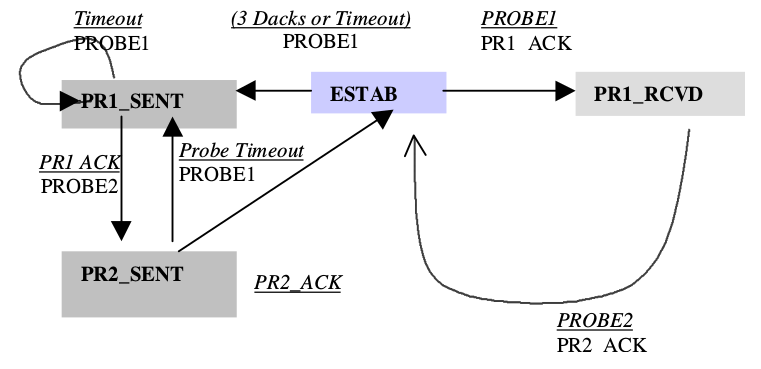
\includegraphics[scale=0.4]{probingDiagram}
    \end{figure}
\end{frame}


\begin{frame}{Open issues}
       \begin{itemize}
	    \item Probe cycles cause more transmission effort.
	    \item The decision-making criteria are conservative
		  because \textit{Immediate Recovery} is entered at the end of
		  probing only in some cases.
	    \item Simply stated, \textit{TCP-Probing}'s
		  behavior is insufficiently aggressive.
       \end{itemize}
\end{frame}




\section{Compound TCP}
\begin{frame}{Issues in High-speed and \newline Long Distance
	      networks}
	\begin{itemize}
		\item Standard TCP can't fully utilize
		      the network capacity because of its
		      conservative approach.
		\item In \textbf{Compound TCP},
		      \textit{delay-based} and \textit{loss-based}
		      approaches coexist.
		\item In \textit{Compound TCP}, a scalable delay-based
		      component is plugged into the
		      \textit{TCP Reno} congestion avoidance algorithm,
		      which is loss-based.
	\end{itemize}
\end{frame}

\begin{frame}{Background}
	\begin{itemize}
	    \item In a \textbf{high-speed} and
		  \textbf{long delay} network, only a
		  very large window can fully utilize the link capacity.
	    \item In real-life networks, a
		  standard TCP sender may never open its window enough
		  to leverage the high-speed resource.
	\end{itemize}
\end{frame}

\begin{frame}{Loss-based vs Delay-based}
	\begin{itemize}
		\item \textbf{Loss-based} strategies modify the increase/decrease parameters
		      in order to become more aggressive. Pitfalls:
			\begin{enumerate}
				\item an aggressive behavior
				      causes more packet losses on bottleneck links;
				\item the throughput of the regular TCP flows is pushed back.
			\end{enumerate}
		\item \textbf{Delay-based} strategies
		      base their decisions on
		      RTT variations (e.g. \textit{FAST-TCP}). They have:
		      \begin{enumerate}
		         \item higher utilization;
		         \item less self-induced packet losses;
		         \item better RTT fairness and stabilization.
		      \end{enumerate}
	\end{itemize}
\end{frame}

\begin{frame}{The Compound TCP (1)}
        \begin{itemize}
		\item Pure delay-based approaches are not competitive to
		      loss-based approaches.
		\item This happens because they reduce their sending rate
		      when bottleneck queue is built. However, this behavior will make
		      loss-based flows increase their sending rate since they
		      notice less packet losses.
        \end{itemize}
\end{frame}


\begin{frame}{The Compound TCP (2)}
        \begin{itemize}
		\item \textit{Compound TCP} incorporates a scalable delay-based component
		      into the standard TCP congestion avoidance algorithm.
		\item Delay-based component's features:
			\begin{enumerate}
				\item rapid window increase
		      	 	      rule when the network is under-utilized;
		      		\item it reduces the sending rate once the bottleneck queue is
		      		      built.
			\end{enumerate}
        \end{itemize}
\end{frame}

\begin{frame}{The Compound TCP (3)}
        \begin{itemize}
		\item A new scalable delay-based component in the 
		      TCP congestion avoidance algorithm is added. 
		\item A new state variable is introduced: \texttt{dwnd} 
		      (\textit{Delay Window}), which controls this delay-based component.
		\item The \texttt{cwnd} remains the same, controlling the loss-based component. 
		\item Thus, the sending window is controlled by both \texttt{cwnd} and \texttt{dwnd}.
	
        \end{itemize}
\end{frame}


\begin{frame}{The Compound TCP (4)}
        \begin{itemize}
		\item \texttt{Sending window = min(cwnd + dwnd, awnd)}.
		\item The \texttt{cwnd} is updated in the same way as in
		      regular TCP's congestion avoidance.
		\item The \textit{Slow-Start} behavior of regular TCP is kept at
		      the start-up of a new connection. In fact,
		      \textit{Slow-Start} is quick
		      enough also for fast and long distance environments.
		\item The delay-based component comes into play
		      in the congestion avoidance phase.
        \end{itemize}
\end{frame}


\begin{frame}{Delay-based component design (1)}
        \begin{itemize}
		\item A state variable (\texttt{baseRTT}) is maintained as
		      an estimation of the delay of a packet over the
		      network path.
		\item A the start of a connection, \texttt{baseRTT} is updated
		      to the minimal observed RTT.
		\item An exponentially smoothed current RTT (\texttt{sRTT}) is also maintained.
        \end{itemize}
\end{frame}


\begin{frame}{Delay-based component design (2)}
        The number of backlogged packets can
	be estimated by means of these formulas:
		\begin{enumerate}
			\item \texttt{expected = win / baseRTT};
			\item \texttt{actual = win / RTT};
			\item \texttt{diff = (expected - actual) * baseRTT}.
		\end{enumerate}
	An early congestion is detected if the number of packets in the queue is larger
	than a fixed threshold $\gamma$ ($diff > \gamma$).
\end{frame}


\begin{frame}{Delay-based component design (3)}
	\begin{enumerate}
		\item Without packet losses:
			$$
				win (t+1) = win(t) + \alpha*win(t)^k
			$$
		\item With packet losses:
			$$
				win (t+1) = win(t) * (1 - \beta)
			$$
	\end{enumerate}
	Parameters $\alpha$, $\beta$ and $k$ should be tuned.
\end{frame}


\begin{frame}{Delay-based component design (4)}
  The delay-based component \texttt{dwnd} is updated following the
  rules below. \newline \newline $dwnd(t+1)$ =
  \center
  \begin{math}
  	\left\{
    	\begin{array}{l}
     		 dwnd (t) + (\alpha*win(t)^k - 1)^+, diff < \gamma\\
      		 (dwnd(t) - \zeta*diff)^+, diff \geq \gamma\\
      		 (win(t)*(1-\beta) - cwnd/2)^+, loss\\
    	\end{array}
  \right.
\end{math}

\end{frame}


\begin{frame}{Open issues}
        \begin{itemize}
		\item The $\gamma$ parameter could be set adaptively.
		\item Early congestion should be detected 
		      by means of constant buffer requirements 
		      regardless of the number of \textit{CTCP} flows.
        \end{itemize}
\end{frame}



\section{Conclusions}
%\input{slides/conclusione}
%\input{slides/problemiRunTime}

\appendix
\section{Bibliography}
\begin{frame}{Bibliography}
	\begin{thebibliography}{10}    
  	\beamertemplatearticlebibitems
  	\bibitem{Goff}
    		T. Goff, J. Moronski, D.S. Phatak, V. Gupta,
		\textit{Freeze-TCP: a true end-to-end TCP enhancement mechanism for 
			  mobile environments}.
  	\bibitem{Tsa}
		V. Tsaoussidis, H. Badr,
		\textit{TCP-probing: towards an error control schema with energy 
		and throughput performance gains}.
	\bibitem{Tan}
		Kun Tan, Jingmin Song, Qian Zhang, Murari Sridharan,
		\textit{A Compound TCP Approach for High-speed and Long Distance Networks}.		
	\end{thebibliography}
\end{frame}

\makethanks
%\renewcommand{\turnOffNumbers}{true} %hide frame numbers in footer

\end{document}
